%----------------------------------------------------------------------------------------
%	POWER CONTROL AND POWER SWITCH.
%----------------------------------------------------------------------------------------
\subsection{Power control \& power switch}


\begin{figure}[H]
\centering
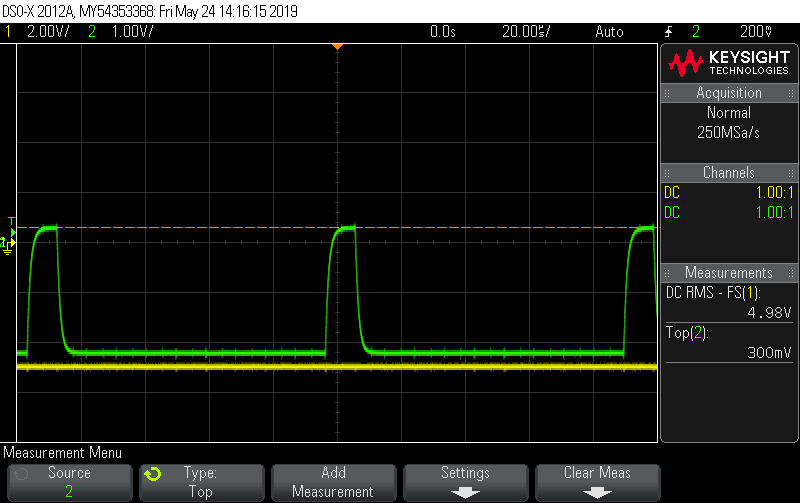
\includegraphics[width=.9\textwidth]{figures/scope_16.png}
\caption{In yellow the input 'TP3' of the power control is shown. In green the output 'TP2' from the pulse generators towards the input of the power control is shown. The voltage does of 'TP2' does not get above $\SI{0.7}{\volt}$ and thus the transistors Q1 and Q2 are inactive.}
\label{fig:scope_16}
\end{figure}


\begin{figure}[H]
\centering
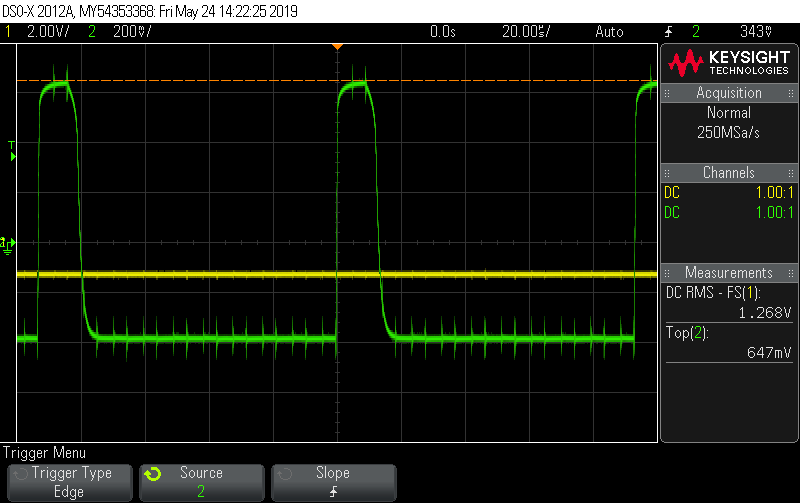
\includegraphics[width=.9\textwidth]{figures/scope_17.png}
\caption{In yellow the input 'TP3' of the power control is shown. In green the output 'TP2' from the pulse generators towards the input of the power control is shown. The reference voltage is increased just over the boundary in order to get the 'TP2' (green) above the $\SI{0.7}{\volt}$ needed to let the diodes D1 and D3 be sperred and the transistors Q1 and Q2 be enabled.}
\label{fig:scope_17}
\end{figure}


\begin{figure}[H]
\centering
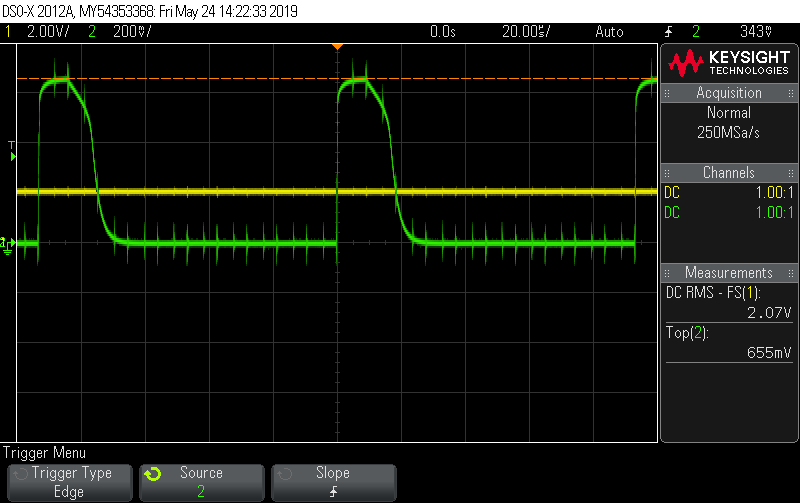
\includegraphics[width=.9\textwidth]{figures/scope_18.png}
\caption{In yellow the input 'TP3' of the power control is shown. In green the output 'TP2' from the pulse generators towards the input of the power control is shown. The reference voltage is further increased, it can be seen that the enable period gets larger.}
\label{fig:scope_18}
\end{figure}

